\section{Preventivo}
La suddivisione oraria viene fatta tenendo conto del fatto che nel corso del progetto ogni  membro del gruppo deve ricoprire ogni ruolo almeno una volta.
Per facilitare la lettura delle successive tabelle sono state utilizzate le seguenti abbreviazioni per identificare i diversi ruoli:
\begin{itemize}
	\item \textbf{Re}: \textit{Responsabile};
	\item \textbf{Am}: \textit{Amministratore};
	\item \textbf{An}: \textit{Analista};
	\item \textbf{Pt}: \textit{Progettista};
	\item \textbf{Pm}: \textit{Programmatore};
	\item \textbf{Ve}: \textit{Verificatore};
\end{itemize}
Inoltre per determinare le ore nulle nelle successive tabelle verrà usato il simbolo -, che ne indica l'assenza.

\subsection{Fase di Analisi}
\subsubsection{Prospetto orario}
Nella fase di Analisi la distribuzione oraria è la seguente:
\begin{table}[H]
	\rowcolors{2}{lightest-grayest}{white}
	\centering
	\renewcommand{\arraystretch}{1.5}
	\begin{tabular}{|c|c|c|c|c|c|c|c|}
		\hline
		\rowcolor{lighter-grayer}
		Nome & Re & Am & An & Pt & Pm & Ve & Totale\\
		\hline
		
		% ----- Modificare da qui -----
		%  collegamento tabella a indice tabelle, dati;
		\hline
		\centering Badan Antonio & \centering & \centering & \centering & \centering & \centering - & \centering & 30 \\
		\hline
		\centering Bertoldo Damiano & \centering & \centering & \centering & \centering & \centering - & \centering & 30 \\
		\hline
		\centering Budai Matteo & \centering & \centering & \centering & \centering & \centering - & \centering & 30 \\
		\hline
		\centering De Grandi Samuele & \centering & \centering & \centering & \centering & \centering - & \centering & 30 \\
		 \hline
		\centering Piacere Ivan & \centering & \centering & \centering & \centering & \centering - & \centering & 30 \\
		 \hline
		\centering Privitera Sara & \centering & \centering & \centering & \centering & \centering - & \centering & 30 \\
		 \hline
		\centering Spigolon Daniele & \centering & \centering & \centering & \centering & \centering - & \centering & 30 \\
		 \hline
		\centering\textbf{Ore totali}  & \centering 25 & \centering 36& \centering 78& \centering 10 & \centering - & \centering 61 & 210 \\
		\hline
		
\end{tabular}
\caption*{\textbf{Tabella 2}: Distribuzione delle ore nella Fase di Analisi\\}
\end{table}	

I dati ottenuti possono essere riassunti nel seguente istogramma:
% fare istogramma (con dati poi), dare titolo e collegare all'indice delle figure;
\\

\subsubsection{Prospetto economico}
In questa fase il costo per ogni ruolo è il seguente:

\begin{table}[H]
	\rowcolors{2}{lightest-grayest}{white}
	\centering
	\renewcommand{\arraystretch}{1.5}
	\begin{tabular}{|c|c|c|}
		\hline
		\rowcolor{lighter-grayer}
		Ruolo & Ore & Costo\\
		\hline
		
		% ----- Modificare da qui -----
		%  collegamento tabella a indice tabelle;
		\centering Responsabile & \centering 25 & 775,00\euro\\ %31 per ora
		\hline
		\centering Amministatore & \centering 36 & 756,00\euro\\ %21 per ora
		\hline
		\centering Analista & \centering 78 & 1950,00\euro\\ %25 per ora
		\hline
		\centering Progettista & \centering 10 & 220,00\euro\\ %22 per ora
		\hline
		\centering Programmatore & \centering - & - \\
		\hline
		\centering Verificatore & \centering 61 & 915,00\euro\\ %15 per ora
		\hline
		\centering\textbf{Totale} & \centering 210 & 4616,00\euro\\
		\hline
\end{tabular}
	\caption*{\textbf{Tabella 3}: Prospetto dei costi per ruolo nella Fase di Analisi\\}
\end{table}
I dati ottenuti possono essere riassunti nel seguente areogramma:
% Dare titolo e collegare all'indice delle figure;
\\
\begin{tikzpicture}
	\pie{11.9/Responsabile, 17.1/Amministartore, 37.1/Analista, 4.8/Progettista, 29.1/Verificatore}
\end{tikzpicture}

	
\subsection{Fase di Consolidamento dei requisiti}
\subsubsection{Prospetto orario}
Nella fase di Consolidamento dei requisiti la distribuzione oraria è la seguente:
\begin{table}[H]
	\rowcolors{2}{lightest-grayest}{white}
	\centering
	\renewcommand{\arraystretch}{1.5}
	\begin{tabular}{|c|c|c|c|c|c|c|c|}
		\hline
		\rowcolor{lighter-grayer}
		Nome & Re & Am & An & Pt & Pm & Ve & Totale\\
		\hline
		
		% ----- Modificare da qui -----
		% collegamento tabella a indice tabelle, dati;
		\centering Badan Antonio & \centering & \centering & \centering & \centering - & \centering - & \centering & 6\\
		\hline
		\centering Bertoldo Damiano & \centering & \centering & \centering & \centering - & \centering - & \centering & 6\\
		\hline
		\centering Budai Matteo & \centering & \centering & \centering & \centering - & \centering - & \centering & 6\\
		\hline
		\centering De Grandi Samuele & \centering & \centering & \centering & \centering - & \centering - & \centering & 6\\
		\hline
		\centering Piacere Ivan & \centering & \centering & \centering & \centering - & \centering - & \centering & 6\\
		\hline
		\centering Privitera Sara & \centering & \centering & \centering & \centering - & \centering - & \centering & 6\\
		\hline
		\centering Spigolon Daniele & \centering & \centering & \centering & \centering - & \centering - & \centering & 6\\
		\hline
		\centering\textbf{Ore totali}  & \centering 3 & \centering 6 & \centering 16& \centering - & \centering - & \centering 17 & 42\\
		\hline
		
\end{tabular}
\caption*{\textbf{Tabella 4}: Distribuzione delle ore nel periodo di Consolidamento dei requisiti\\}
\end{table}	
I dati ottenuti possono essere riassunti nel seguente istogramma:
% fare istogramma (con dati poi), dare titolo e collegare all'indice delle figure;
\\

\subsubsection{Prospetto economico}
In questa fase il costo per ogni ruolo è il seguente:

\begin{table}[H]
	\rowcolors{2}{lightest-grayest}{white}
	\centering
	\renewcommand{\arraystretch}{1.5}
	\begin{tabular}{|c|c|c|}
		\hline
		\rowcolor{lighter-grayer}
		Ruolo & Ore & Costo\\
		\hline
		% Manca centrare ultima colonna, titolo tabella, collegamento tabella a indice tabelle, dati;
		\centering Responsabile & \centering 3 & 93,00\euro\\
		\hline
		\centering Amministatore & \centering 6 & 126,00\euro\\
		\hline
		\centering Analista & \centering 16 & 400,00\euro\\
		\hline
		\centering Progettista & \centering - & -\\
		\hline
		\centering Programmatore & \centering - & - \\
		\hline
		\centering Verificatore & \centering 17 & 255,00\euro\\
		\hline
		\centering\textbf{Totale} & \centering 42 & 874,00\euro\\
		\hline
		\end{tabular}
\caption*{\textbf{Tabella 5}: Prospetto dei costi per ruolo nel periodo di Consolidamento dei requisiti\\}
\end{table}

I dati ottenuti possono essere riassunti nel seguente areogramma:
%Dare titolo e collegare all'indice delle figure;
\\
\begin{tikzpicture}
	\pie{7.1/Responsabile, 14.3/Amministratore, 38.1/Analista, 40.5/Verificatore}
\end{tikzpicture}



\subsection{Fase di Progettazione architetturale}
\subsubsection{Prospetto orario}

\subsubsection{Prospetto economico}

\subsection{Fase di Progettazione di dettaglio e codifica}
\subsubsection{Prospetto orario}

\subsubsection{Prospetto economico}

\subsection{Fase di Validazione e collaudo}
\subsubsection{Prospetto orario}
Nella fase di Validazione e collaudo la distribuzione oraria è la seguente:

\begin{table}[H]
	\rowcolors{2}{lightest-grayest}{white}
	\centering
	\renewcommand{\arraystretch}{1.5}
	\begin{tabular}{|c|c|c|c|c|c|c|c|}
		\hline
		\rowcolor{lighter-grayer}
		Nome & Re & Am & An & Pt & Pm & Ve & Totale ore\\
		\hline
		Badan Antonio & 4 & 0 & 0 &  10 & 4 & 7 & 25 \\
		\hline
		Bertoldo Damiano & 6 & 0 & 0 & 0 & 10 & 9 & 25 \\
		\hline
		Budai Matteo & 0 & 9 & 0 & 0 & 5 & 11 & 25 \\
		\hline
		De Grandi Samuele & 0 & 7 & 0 & 5 & 4 & 9 & 25 \\
		\hline
		Piacere Ivan & 0 & 8 & 0 & 0 & 4 & 13 & 25 \\
		\hline
		Privitera Sara & 6 & 0 & 0 & 10 & 6 & 3 & 25 \\
		\hline
		Spigolon Daniele & 4 & 0 & 0 & 0 & 10 & 11 & 25 \\
		\hline
		Ore totali & 20 & 24 & 0 & 25 & 43 & 63 & 175 \\
		\hline
	\end{tabular}
	\caption*{\textbf{Tabella 15}: Distribuzione delle ore nel periodo di Validazione e collaudo\\}
\end{table}	
	I dati ottenuti possono essere riassunti nel seguente istogramma:

\begin{figure}[H]
	\centering
	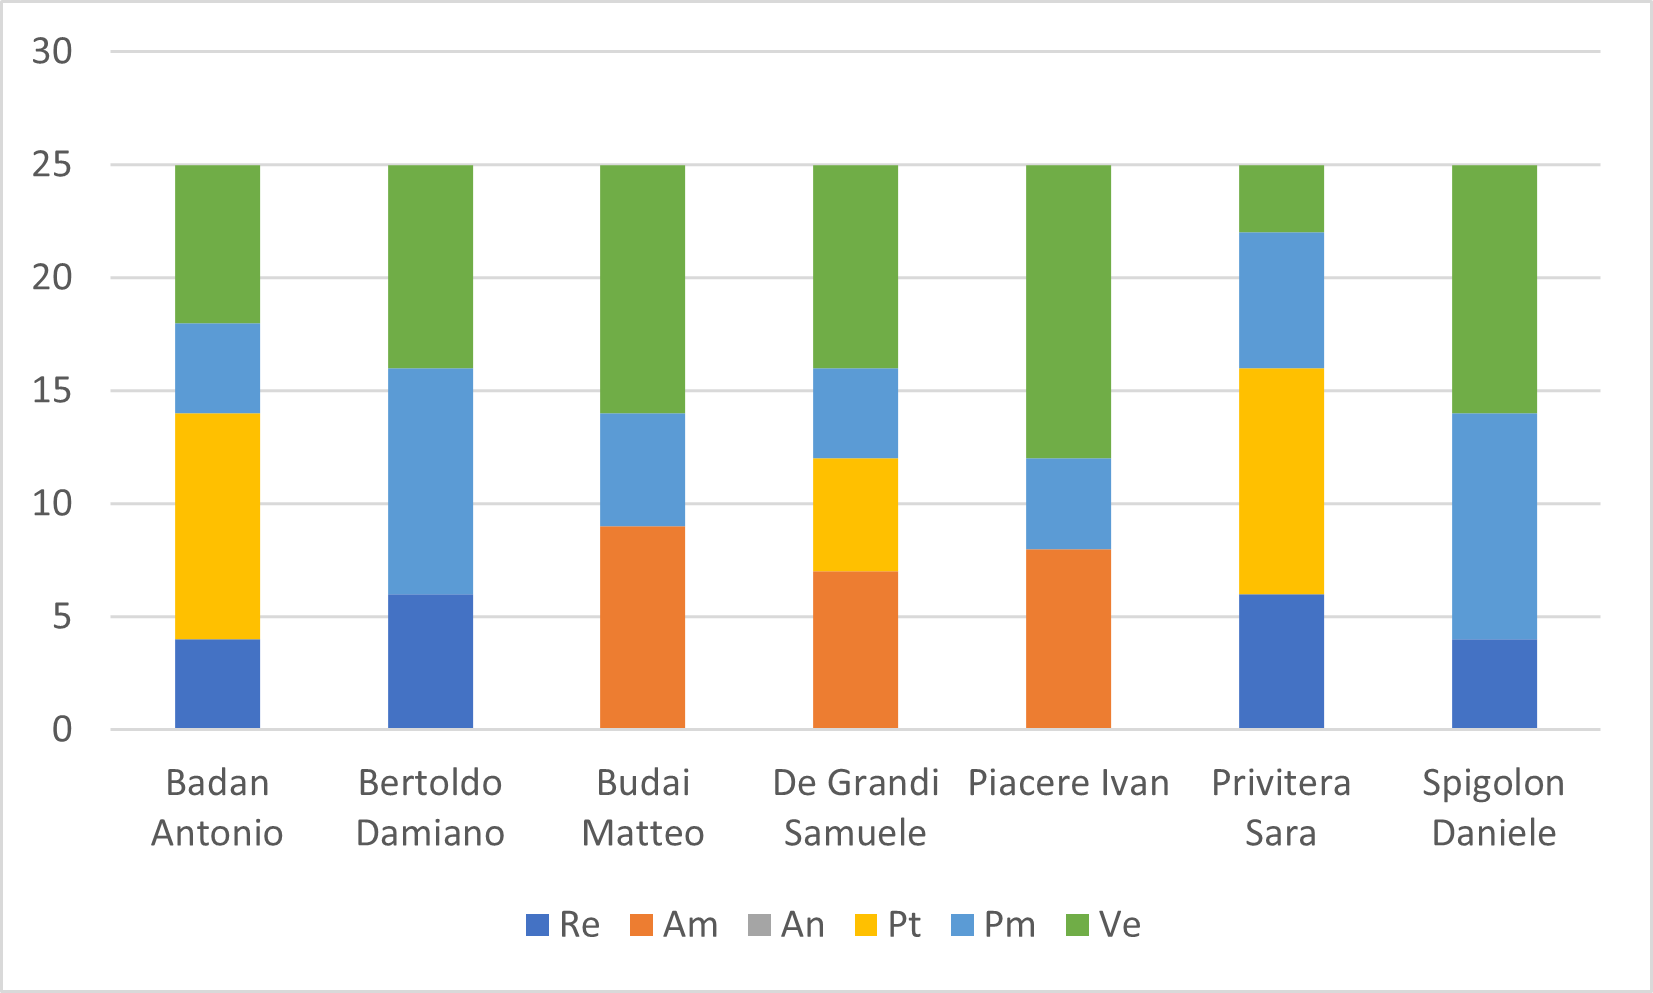
\includegraphics[width=0.7\linewidth]{res/images/Figura11.png}
	\caption*{\textbf{Figura11}: Istogramma della suddivisione delle ore durante il periodo di Validazione e collaudo}
	\label{fig:Figura10}
\end{figure}
	
	
\subsubsection{Prospetto economico}
In questa fase il costo per ogni ruolo è il seguente:

\begin{table}[H]
	\rowcolors{2}{lightest-grayest}{white}
	\centering
	\renewcommand{\arraystretch}{1.5}
	\begin{tabular}{|c|c|c|}
		\hline
		\rowcolor{lighter-grayer}
		Ruolo & Ore & Costo \\
		\hline
		Responsabile & 20 & 620\euro \\
		\hline
		Amministratore & 24 & 504\euro \\
		\hline
		Analista & 0 & 0\euro \\
		\hline
		Progettista & 25 & 550\euro \\
		\hline
		Programmatore & 43 & 946\euro \\
		\hline
		Verificatore & 63 & 945\euro \\
		\hline
		Totale & 175 &  3565\euro \\
		\hline
	\end{tabular}
\caption*{\textbf{Tabella 16}: Prospetto dei costi per ruolo nel periodo di Validazione e collaudo\\}
\end{table}

I dati ottenuti possono essere riassunti nel seguente areogramma:


\begin{figure}[!h]
	\centering
	\begin{tikzpicture}
		\pie{11.9/Responsabile, 17.1/Amministratore, 37.1/Analista, 4.8/Progettista, 29.1/Verificatore}
	\end{tikzpicture}
	\caption*{\textbf{Figura 10}: Areogramma della ripartizione di ore per ruolo in Validazione e collaudo}
	\label{fig:Figura10}
\end{figure}

\subsection{Riepilogo}
\subsubsection{Ore totali}
\paragraph{Prospetto orario totale}
Nella seguente tabella viene riportata la distribuzione oraria di tutte le fasi:

\begin{table}[H]
	\rowcolors{2}{lightest-grayest}{white}
	\centering
	\renewcommand{\arraystretch}{1.5}
	\begin{tabular}{|c|c|c|c|c|c|c|c|}
		\hline
		\rowcolor{lighter-grayer}
		Nome & Re & Am & An & Pt & Pm & Ve & Totale ore\\
		\hline
		Badan Antonio &  &  &  &  &  &  & 20 \\
		\hline
		Bertoldo Damiano&  &  &  &  &  &  & 20 \\
		\hline
		Budai Matteo&  &  &  &  &  &  & 20 \\
		\hline
		De Grandi Samuele&  &  &  &  &  &  & 20 \\
		\hline
		Piacere Ivan&  &  &  &  &  &  & 20 \\
		\hline
		Privitera Sara&  &  &  &  &  &  & 20 \\
		\hline
		Spigolon Daniele&  &  &  &  &  &  & 20 \\
		\hline
		Ore totali&  &  &  &  &  &  & 120 \\
		\hline
	\end{tabular}
	\caption*{\textbf{Tabella 15}: Prospetto orario che comprende tutte le fasi trattate in precedenza\\}
\end{table}	
I dati ottenuti possono essere riassunti nel seguente istogramma:

\begin{figure}[H]
	\centering
	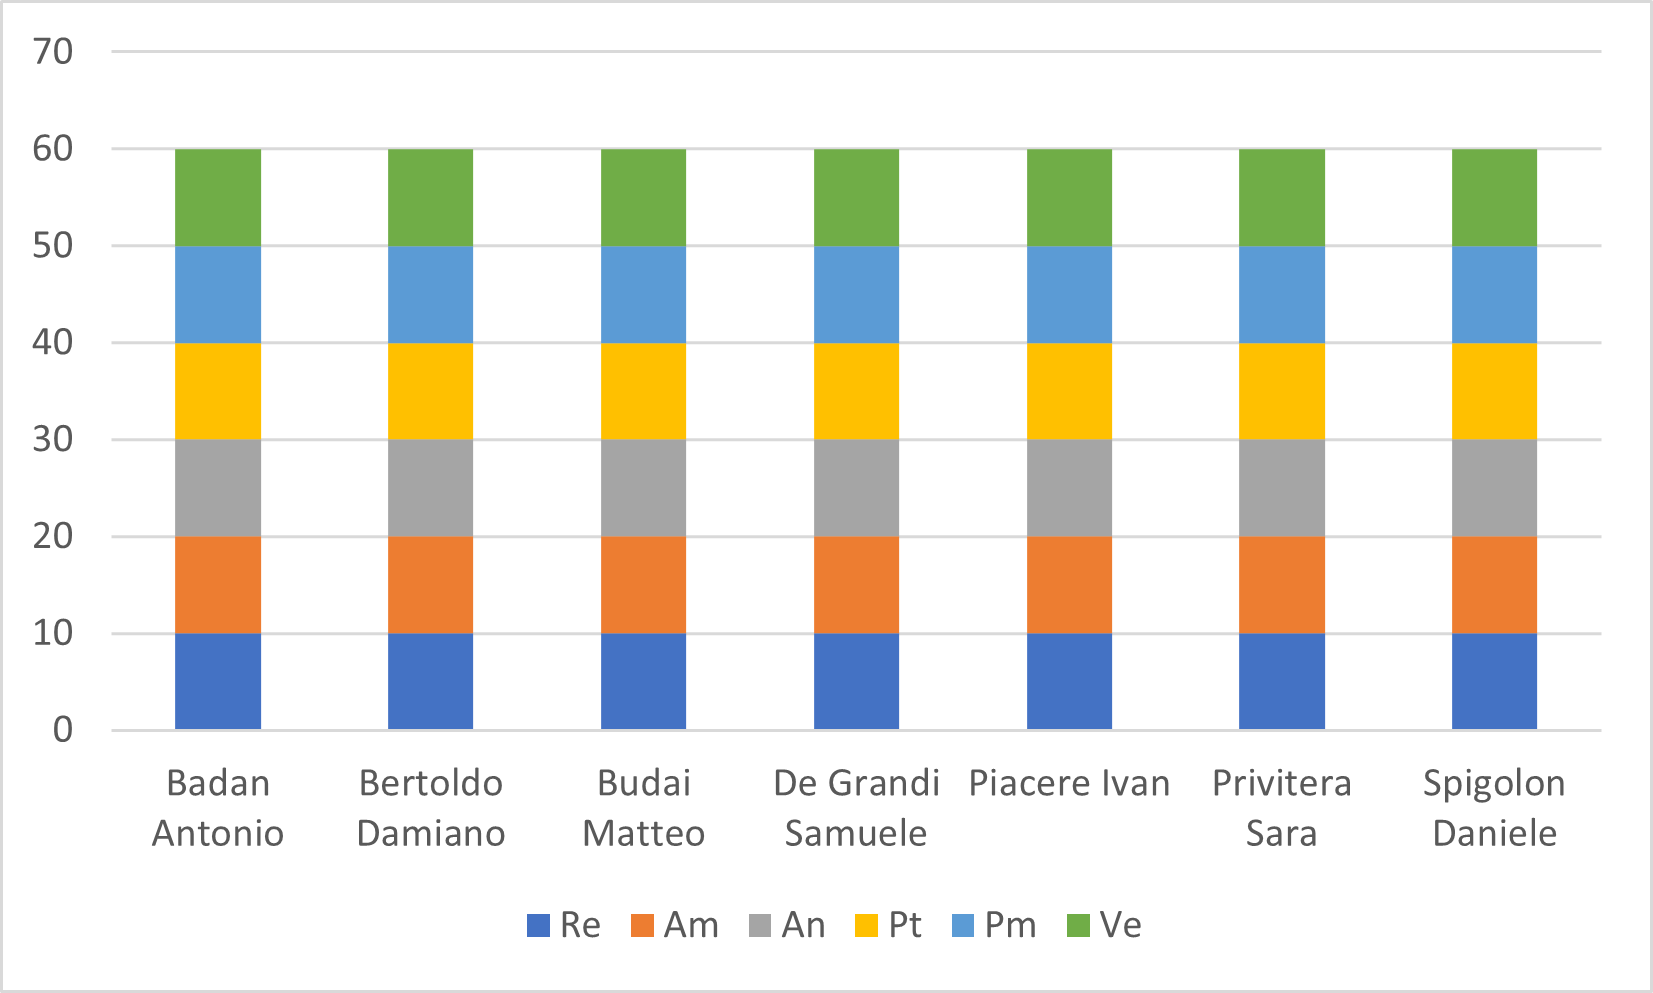
\includegraphics[width=0.7\linewidth]{res/images/Figura10.png}
	\caption*{\textbf{Figura10}: Istogramma della suddivisione delle ore di tutte le fasi trattate in precedenza}
	\label{fig:Figura10}
\end{figure}

\paragraph{Prospetto economico totale}
Nella seguente tabella vengono mostrati i costi complessivi per ogni ruolo:

\begin{table}[H]
	\rowcolors{2}{lightest-grayest}{white}
	\centering
	\renewcommand{\arraystretch}{1.5}
	\begin{tabular}{|c|c|c|}
		\hline
		\rowcolor{lighter-grayer}
		Ruolo & Ore & Costo \\
		\hline
		Responsabile &  &  \\
		\hline
		Amministratore &  &  \\
		\hline
		Analista &  &  \\
		\hline
		Progettista&  &  \\
		\hline
		Programmatore &  &  \\
		\hline
		Verificatore &  & 50\euro \\
		\hline
		Totale &  &  800,00\euro \\
		\hline
	\end{tabular}
	\caption*{\textbf{Tabella 16}: Prospetto dei costi totali per ciascun ruolo \\}
\end{table}

I dati ottenuti possono essere riassunti nel seguente areogramma:


\begin{figure}[!h]
	\centering
	\begin{tikzpicture}
		\pie{11.9/Responsabile, 17.1/Amministratore, 37.1/Analista, 4.8/Progettista, 29.1/Verificatore}
	\end{tikzpicture}
	\caption*{\textbf{Figura 10}: Areogramma dei costi totali delle ore di investimento e rendicontate}
    \label{fig:Figura10}
\end{figure}

\subsubsection{Ore totali rendicontate}
\paragraph{Prospetto orario totale rendicontato}
Nella seguente tabella viene riportata la distribuzione oraria di tutte le fasi a carico del committente, ad esclusione quindi, dell'Analisi e del Consolidamento dei requisiti:

\begin{table}[H]
	\rowcolors{2}{lightest-grayest}{white}
	\centering
	\renewcommand{\arraystretch}{1.5}
	\begin{tabular}{|c|c|c|c|c|c|c|c|}
		\hline
		\rowcolor{lighter-grayer}
		Nome & Re & Am & An & Pt & Pm & Ve & Totale ore\\
		\hline
		Badan Antonio &  &  &  &  &  &  & 20 \\
		\hline
		Bertoldo Damiano&  &  &  &  &  &  & 20 \\
		\hline
		Budai Matteo&  &  &  &  &  &  & 20 \\
		\hline
		De Grandi Samuele&  &  &  &  &  &  & 20 \\
		\hline
		Piacere Ivan&  &  &  &  &  &  & 20 \\
		\hline
		Privitera Sara&  &  &  &  &  &  & 20 \\
		\hline
		Spigolon Daniele&  &  &  &  &  &  & 20 \\
		\hline
		Ore totali&  &  &  &  &  &  & 120 \\
		\hline
	\end{tabular}
	\caption*{\textbf{Tabella 15}: Prospetto orario che comprende tutte le ore rendicontate\\}
\end{table}	
I dati ottenuti possono essere riassunti nel seguente istogramma:

\begin{figure}[H]
	\centering
	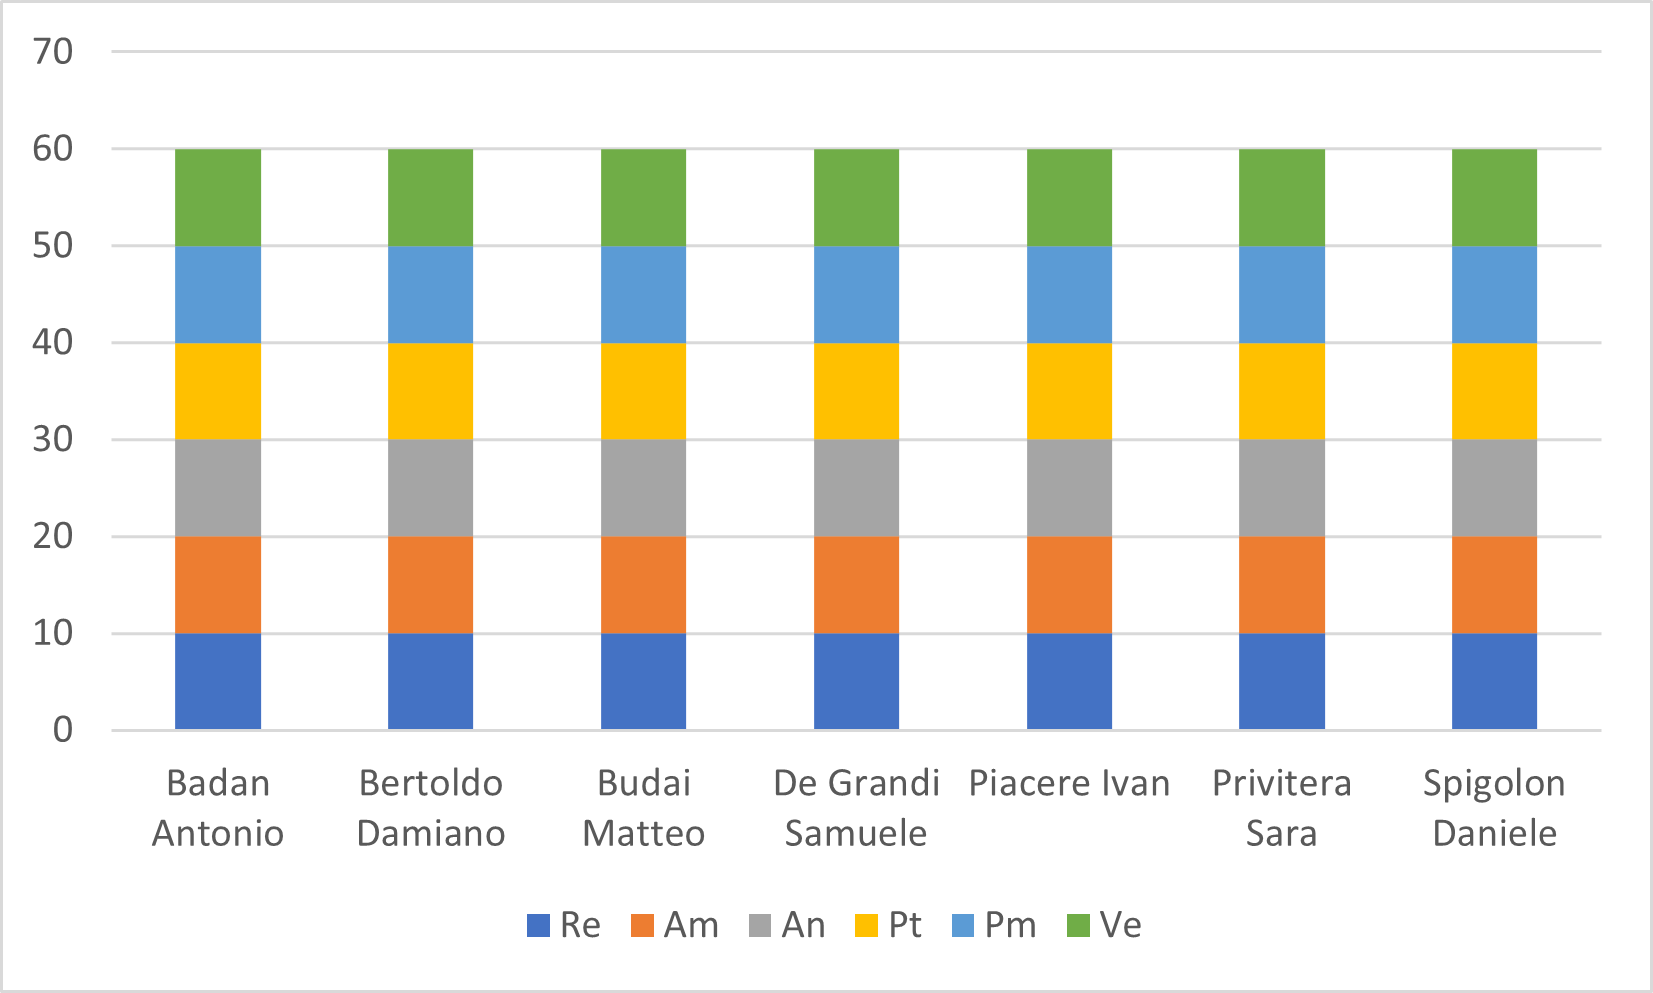
\includegraphics[width=0.7\linewidth]{res/images/Figura10.png}
	\caption*{\textbf{Figura10}: Istogramma della suddivisione delle ore rendicontate}
	\label{fig:Figura10}
\end{figure}

\paragraph{Prospetto economico totale rendicontato}
Nella seguente tabella vengono mostrati i costi complessivi rendicontati per ogni ruolo:

\begin{table}[H]
	\rowcolors{2}{lightest-grayest}{white}
	\centering
	\renewcommand{\arraystretch}{1.5}
	\begin{tabular}{|c|c|c|}
		\hline
		\rowcolor{lighter-grayer}
		Ruolo & Ore & Costo \\
		\hline
		Responsabile &  &  \\
		\hline
		Amministratore &  &  \\
		\hline
		Analista &  &  \\
		\hline
		Progettista&  &  \\
		\hline
		Programmatore &  &  \\
		\hline
		Verificatore &  & 50\euro \\
		\hline
		Totale &  &  800,00\euro \\
		\hline
	\end{tabular}
	\caption*{\textbf{Tabella 16}: Prospetto dei costi totali rendicontati \\}
\end{table}

I dati ottenuti possono essere riassunti nel seguente areogramma:


\begin{figure}[!h]
	\centering
	\begin{tikzpicture}
		\pie{11.9/Responsabile, 17.1/Amministratore, 37.1/Analista, 4.8/Progettista, 29.1/Verificatore}
	\end{tikzpicture}
	\caption*{\textbf{Figura 10}: Areogramma delle ore rendicontate per ruolo}
    \label{fig:Figura10}
\end{figure}

\subsubsection{Conclusioni}
Il costo del progetto considerando le ore rendicontate è: \euro.